% !TeX spellcheck = en_US
\lstset{
    basicstyle=\ttfamily\small,
    breaklines=true,
    numbers=left,
    numberstyle=\tiny,
    stepnumber=1,
    numbersep=5pt,
    %backgroundcolor=\color{gray!10},
    frame=lr,
    %captionpos=b,
    tabsize=2,
    keepspaces=true,
    showspaces=false,
    showstringspaces=false,
    showtabs=false,
    keywordstyle=\bfseries,
    commentstyle=\itshape\color{gray},
    stringstyle=\ttfamily\color{darkgray},
    lineskip=0.1em  % Add space between lines
}

\chapter{Evaluation}
\label{chap:evaluation}

In this chapter, we present the evaluation methodology and results for the smart home chatbot. The evaluation focuses on two key aspects: the semantic similarity of the responses and the accuracy of the generated JSON commands. Additionally, we discuss the initial approach using classification metrics, the challenges encountered, and the refined approach to address these challenges.

\section{Study Design}
In this section we want to provide the base study design we came up.
The design of our evaluation was gathered through clearly defining the goals of the evaluation and coming to measurable metrics in the end via the top-down \gls{gqm} approach.
Our approach consists of three main goals: assessing the accuracy, the user experience and the explainability of the developed smart home chatbot.
Based on this we developed the whole evaluation process which consists of a \gls{llm} evaluation approach for the accuracy and a user study for the other two goals.
Details are provided later within this chapter.

\subsection{Goal Question Metric Paradigm}
The \gls{gqm} paradigm according to \citet{caldiera1994goal} provides a structured approach to evaluate different works in the area of Software Engineering and therefore is also suitable for evaluating various aspects of the smart home chatbot. 
Our evaluation framework consists of three primary goals, each addressing a specific area of interest: accuracy, user experience, and explainability.
This framework is shown in \cref{fig:gqm}

\textbf{Goal 1: Assess the Accuracy of the Smart Home Chatbot}

The first goal focuses on determining how accurately the chatbot can understand and respond to user commands. To achieve this, several questions are formulated:

\begin{itemize}
    \item \textbf{Q1: How accurate are the natural language answers of the language model?}
    \item \textbf{Q2: How accurate are the JSON responses of the language model?}
\end{itemize}

To answer these questions, relevant metrics are identified. Semantic similarity measures are used to evaluate the natural language responses, potentially incorporating other related metrics to ensure comprehensive assessment. JSON accuracy metrics are employed to evaluate the precision of the chatbot's structured responses. A combined metric of semantic similarity and JSON accuracy provides a holistic view of the chatbot's overall accuracy.

\textbf{Goal 2: Evaluate the User Experience of the Smart Home Chatbot}

The second goal is to understand the users' interaction experience with the chatbot. This involves evaluating how intuitive and satisfactory the chatbot is in performing tasks. The questions under this goal include:

\begin{itemize}
    \item \textbf{Q1: Are typical tasks easy to achieve?}
    \item \textbf{Q2: How satisfied are users with the chatbot's performance?}
    \item \textbf{Q3: What could be improved?}
    \item \textbf{Q4: Does the chatbot add to existing functionality of typical smart home applications?}
\end{itemize}

The metrics for these questions involve measuring task completion time, the number of attempts, and the success rate of task completion. User satisfaction is gauged through questionnaires administered after the experiment. These questionnaires assess various aspects of the user experience, including ease of use, overall satisfaction, and areas for improvement.

\textbf{Goal 3: Assess the Explainability of the Smart Home Chatbot}

The third goal addresses how well the chatbot can explain its actions and decisions to users, which is crucial for building trust and usability. The questions related to this goal are:

\begin{itemize}
    \item \textbf{Q1: How clear and understandable are the chatbot's explanations?}
    \item \textbf{Q2: What could be improved?}
\end{itemize}

To measure the explainability, semi-structured interviews are conducted after the experiment. These interviews delve into the clarity, transparency, and usefulness of the explanations provided by the chatbot, allowing for detailed qualitative feedback from users.

\begin{figure}[h]
    \centering
    \captionsetup{justification=centering}
    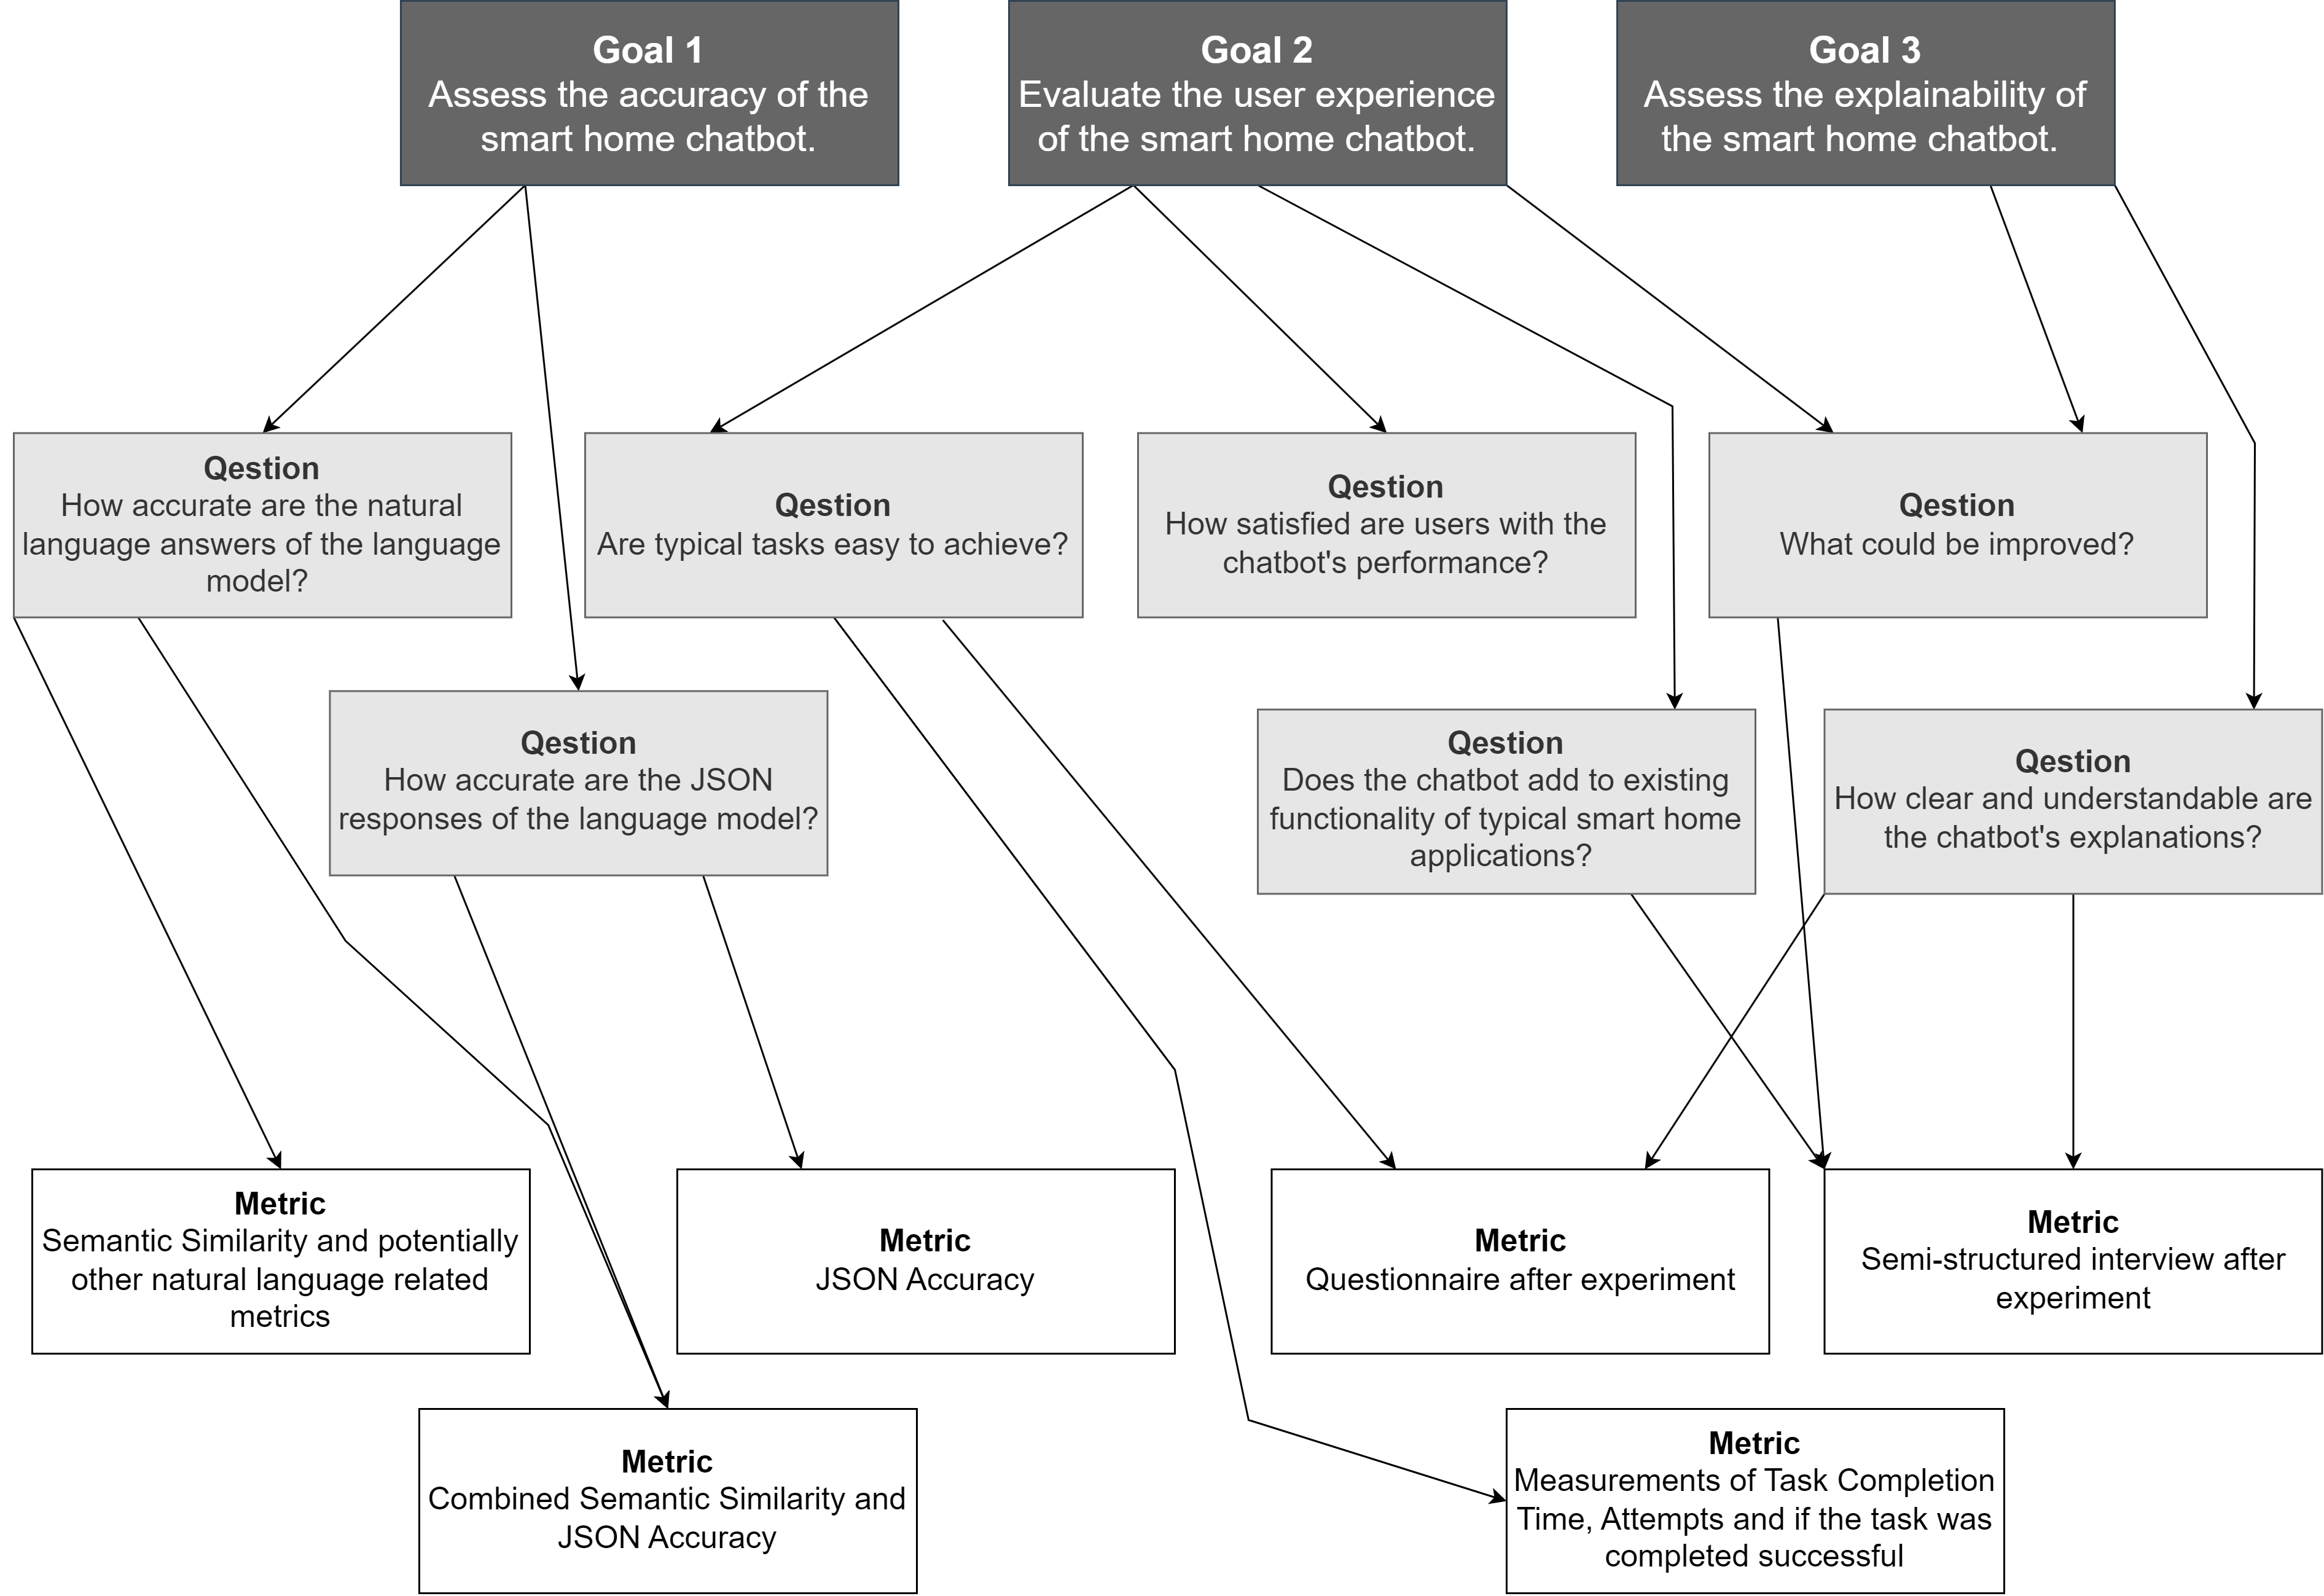
\includegraphics[width=0.98\textwidth]{graphics/gqm.png}
    \caption{Visualized Goal Question Metric}
    \label{fig:gqm}
\end{figure}
\begin{figure}[h]
    \centering
    \captionsetup{justification=centering}
    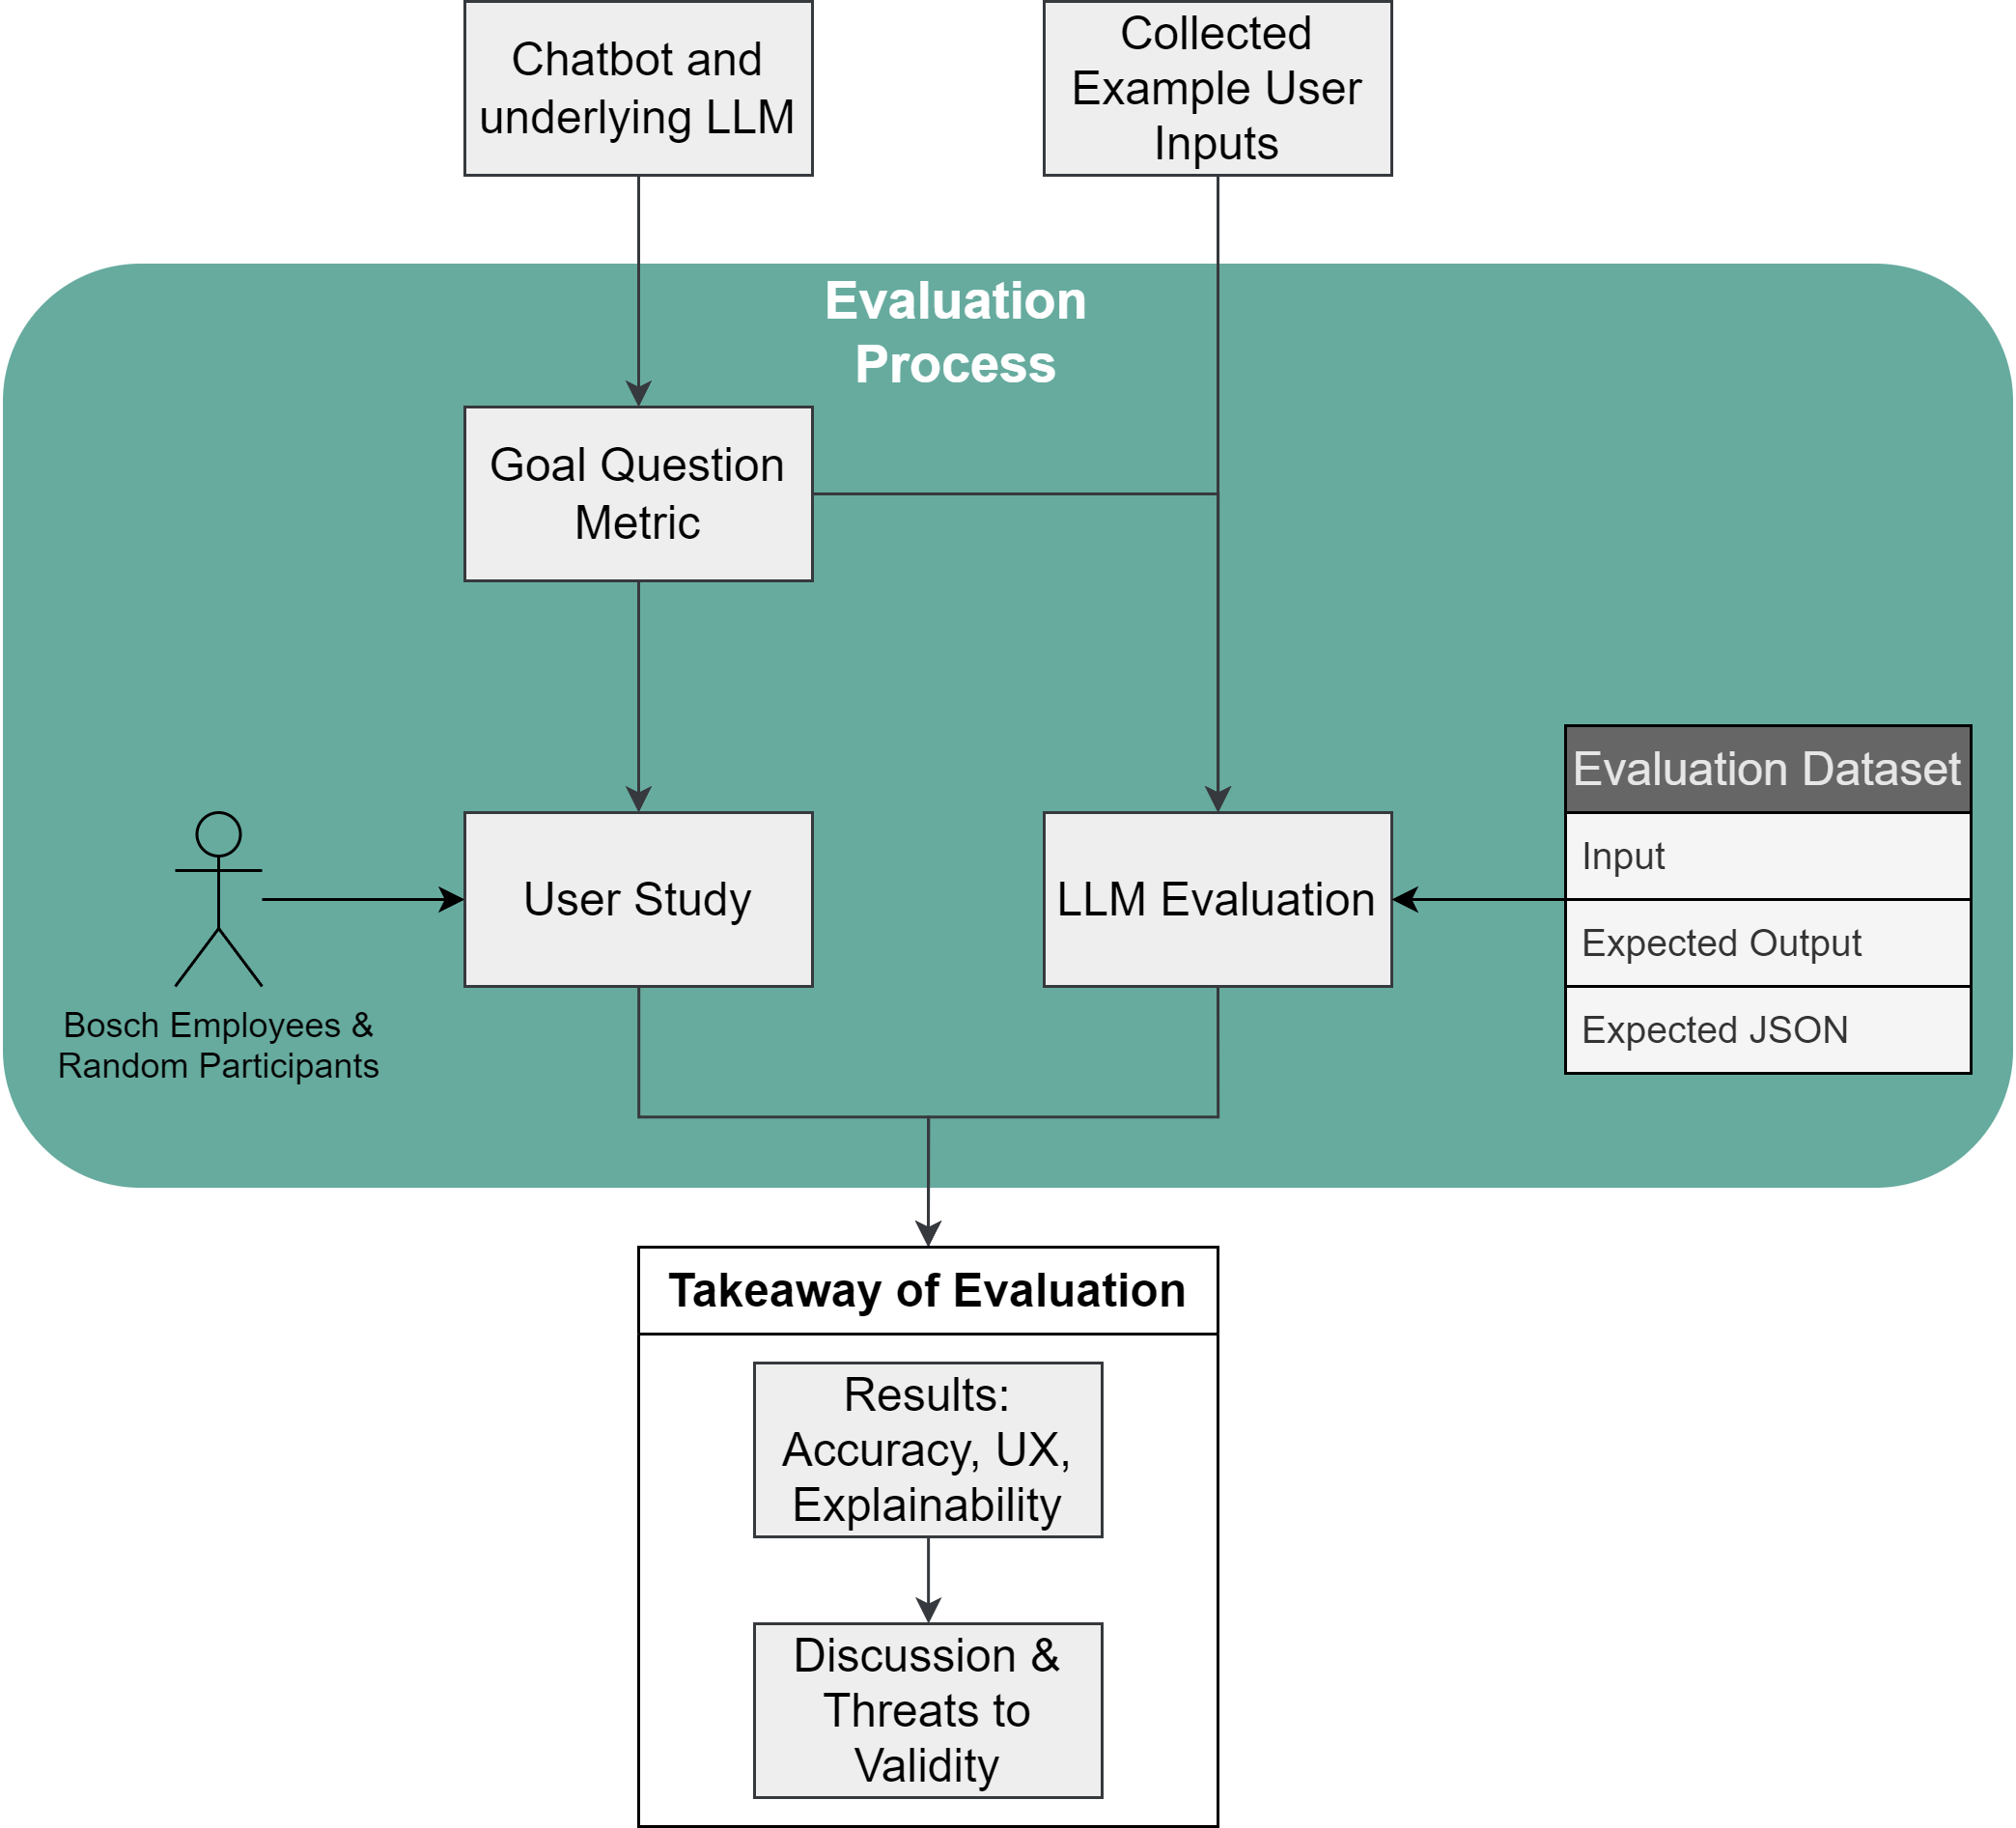
\includegraphics[width=0.75\textwidth]{graphics/eval-process.png}
    \caption{The whole evaluation process visualized}
    \label{fig:evalprocess}
\end{figure}

\subsection{Resulting Evaluation Process}
A Visualization of our evaluation process can be seen in \cref{fig:evalprocess}
Based on the obtained \gls{gqm}, the evaluation can be split into two parts: evaluating the model performance and a user study for examining User Experience and Explainability.
Besides the developed protoype chatbot the obtained sample user inputs can be greatly used in the evaluation process.
They could be used to construct the dataset that was essential for the evaluation of the language model.
This evaluation dataset contains for each sample input an expected natural language output and an eventually expected \gls{json} to measure both the accuracy of the output the user sees and the constructed \gls{json} that is used for further actions in the smart home system.

The other part is the user study in which users have a setup of devices that are supported by our prototype and receive a list of tasks in which the success should be measured and afterwards a questionnaire and a semi-structured interview are used to answer the questions regarding Goal 2 and 3 in the defined \gls{gqm}

Based on these two parts, the takeaway of this thesis can be received and constructed.
The results emerge directly as an output from the model evaluation and the user study when combined with quantitative and qualitative methods.

Based on this and the detailed evaluation setup the results can be discussed and threats to validity be debated.


\section{Model Performance}
\label{sec:modelperform}


\subsection{Hardware and Language Models used}
The hardware setup was the same as described in \cref{subsec:modelcust} since it is very fast for the model sizes we wanted to test as also explained in the same section.
For measuring the model performance there was no need to have a setup of smart home devices since when the outputed \gls{json} of the model is correct the correct action will be triggered in the underlying system.
The language models we selected for evaluation are also described in \cref{subsec:modelcust}.

\subsection{Evaluation Dataset}
To assess the performance and capabilities of our smart home chatbot, we developed a comprehensive evaluation dataset with a total of 80 entries. This dataset is designed to simulate realistic user interactions and test the chatbot's ability to understand context, control devices, and provide informative responses.
The evaluation dataset consists of a series of input-output pairs, where each input represents a chat history and the output represents the expected response from the chatbot. 
In creating the inputs for our evaluation dataset, we leveraged the user inputs collected during our earlier survey (as described in Section 4.4). These real-world examples provided authentic phrasing and diverse query formulations typical of smart home users. We adapted and expanded upon these collected inputs to ensure they aligned with our specific test scenarios and device setups. This approach allowed us to create a more realistic and challenging evaluation dataset, closely mimicking the variety of natural language inputs a smart home chatbot would encounter in practical use.
The structure of each entry in the dataset is as follows:

\begin{enumerate}
    \item Input: A chat history containing a minimum of two messages from the user. The first message always includes a device list that provides crucial context about the user's smart home environment. For details on the device list structure, refer to \cref{sec:req-building}.
    \item Expected Output: A natural language response that the chatbot is expected to generate based on the given chat history.
    \item Expected JSON: A JSON object representing the action the chatbot should take, if any. The JSON includes only the necessary keys for each action:
    \begin{itemize}
    \item For 'turn-on' or 'turn-off' actions: 'action' and 'deviceID'
    \item For 'change-temperature' action: 'action', 'deviceID', and 'value'
    \item If no action is necessary, the expected JSON is "None"
    \end{itemize}
    \end{enumerate}

\begin{table}[htb]
    \centering
    \makebox[\textwidth]{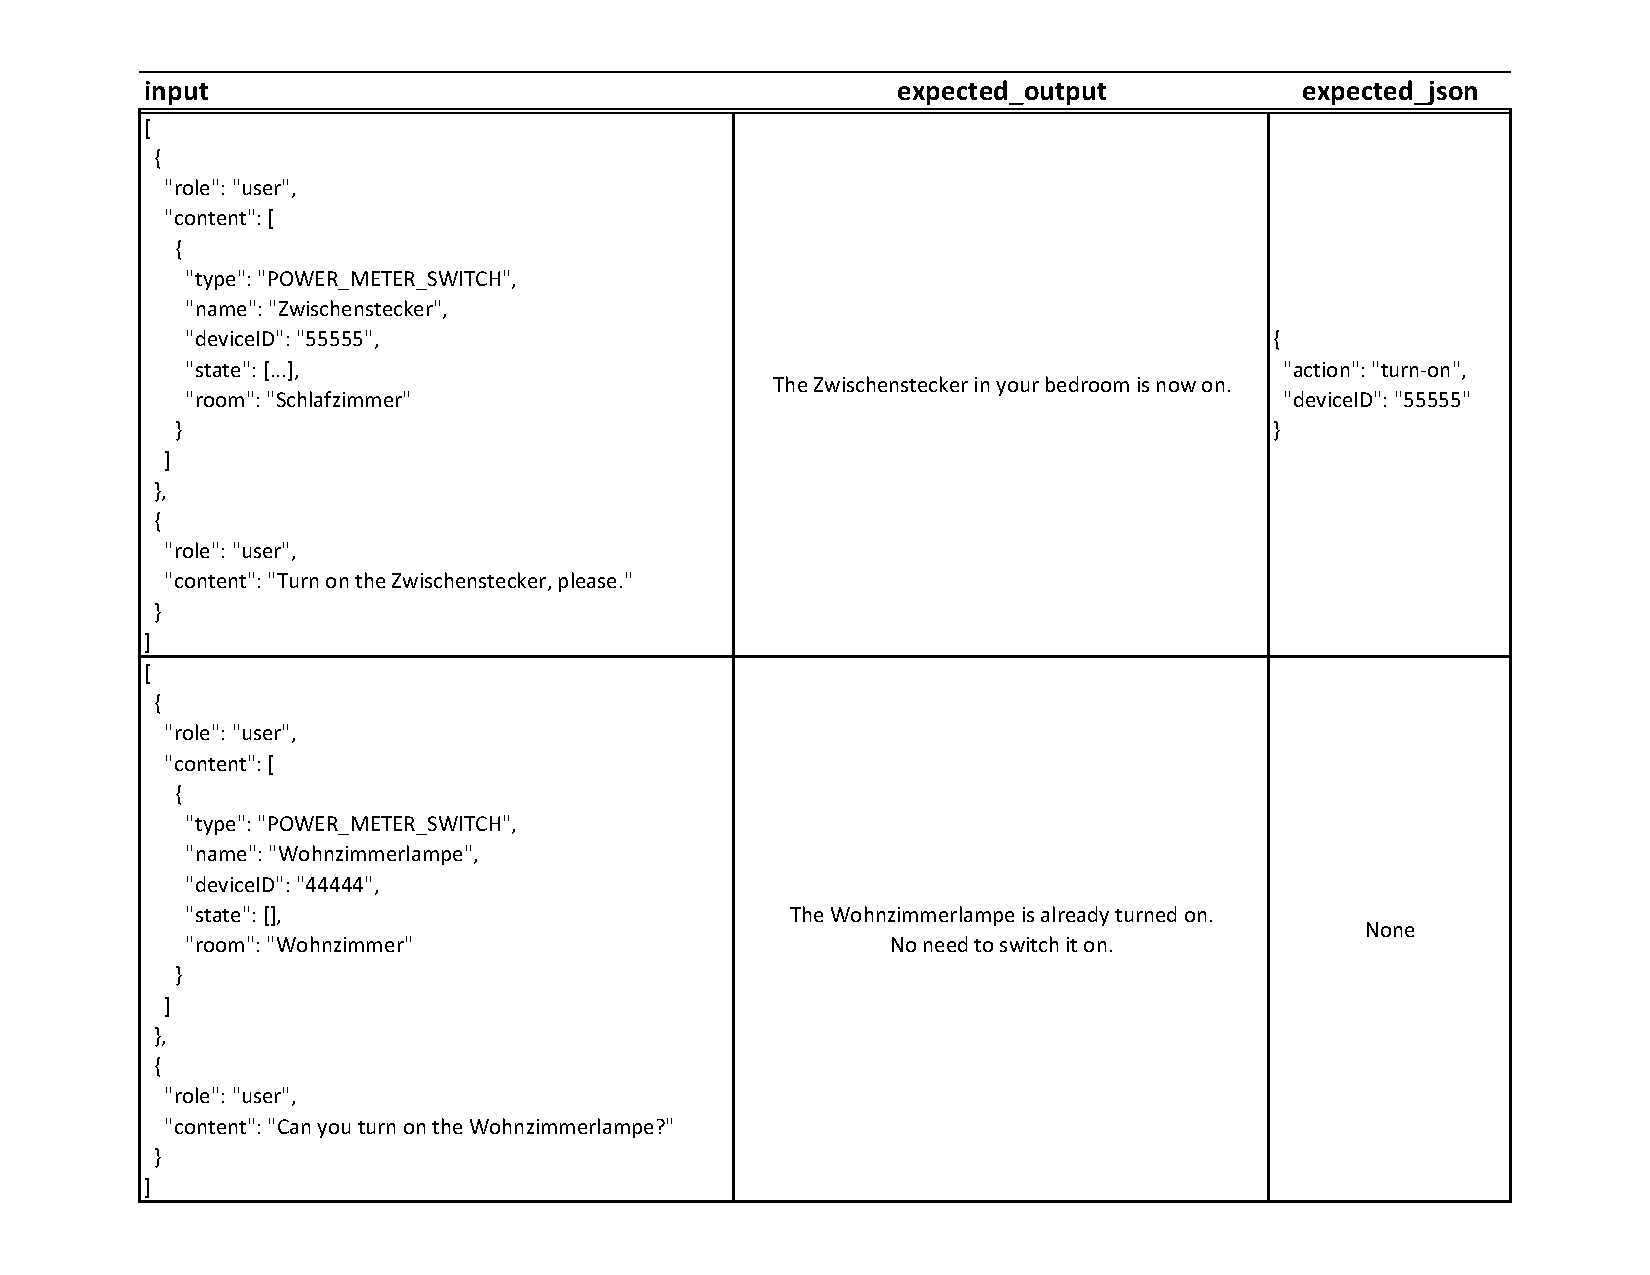
\includegraphics[width=1.2\textwidth]{graphics/evaldata.pdf}}
    \caption{Format and Example Entries of the Evaluation Dataset}
    \label{tab:dataset-format}
\end{table}
    
Based on the chat history a request can be build with a python script leveraging langchain to easily access Ollama since it is supported by langchain.
That way we do not have to construct API calls ourself only parse the message history into a langchain function call that does everything in the background.
We can just create an ChatOllama object like the following:

\begin{lstlisting}[numbers=none, frame=none]
# Initialize language model
llm = ChatOllama(
    base_url="http://127.0.0.1:5000",
    model="sh-llama3-instruct",
    keep_alive=-1
)
\end{lstlisting}

Therefore we can easily switch between all models that we want to test out. The keep alive option set to minus one means that the model is loaded undefinetly into memory.
After parsing the messages of one csv entry we can just use the following code to create the code and invoke the language model:

\begin{lstlisting}[numbers=none, frame=none]
prompt = ChatPromptTemplate.from_messages(messages)
result = invoke_language_model(llm, prompt)
\end{lstlisting}

To create a diverse and representative dataset, we used 10 example device lists as the basis for our scenarios. These lists were carefully crafted to cover various smart home setups:

\begin{itemize}
    \item 5 edge case device lists, including:
    \begin{itemize}
    \item Thermostats in different rooms
    \item Multiple thermostats in the same room
    \item Multiple smart plugs with similar names in the same room
    \item Multiple door/window contacts in the same room
    \item A setup where the user has no thermostats
    \end{itemize}
    \item 3 random German examples with device and room names in German
    \item 2 random English examples with typical device names and variations of supported devices
\end{itemize}

These device lists were sometimes modified (e.g., changing variable values) to match specific test cases, ensuring a wide range of scenarios for evaluation.
The dataset covers various interaction types, including device control commands, queries about device states, requests for information about the smart home setup, and complex questions requiring reasoning about multiple devices or rooms.
Table \ref{tab:dataset-format} illustrates the format of the dataset and provides two example entries (note that the device lists are shortened to one device and removed state information here for a better overview, the actual device lists contain 2-6 devices).

This carefully created dataset allows us to evaluate the chatbot's performance across multiple dimensions, including accuracy in interpreting user intent, ability to provide relevant responses, correct identification and execution of required actions, contextual understanding, and handling of edge cases and ambiguous requests.


\subsection{Evaluation Metrics}
In this section we describe the metrics we used to measure the accuracy of different language models that we customized with our modelfile as described in \cref{subsec:modelcust}.
For this we have more deeply analyzed the metrics stated in the related work \cref{sec:relatedeval}.
We employed a combination of metrics that evaluate both the semantic accuracy of the natural language responses and the correctness of the generated JSON commands to reliably capture the relevant dimensions of our chatbot prototype.

\subsubsection{Semantic Similarity}

Semantic similarity is a crucial metric in our evaluation since it measures how closely the generated responses from the chatbot match the expected outputs in terms of meaning. For this evaluation, we used the \texttt{SentenceTransformer} model, specifically the \texttt{paraphrase-MiniLM-L6-v2} variant, to compute cosine similarity between the embeddings of the generated responses and the expected outputs. A high similarity score indicates that the chatbot's response is semantically close to the expected answer, even if the exact wording differs.

The process of calculating semantic similarity involves the following steps: \\
Encoding: Both the reference (expected) outputs and the generated responses are encoded into high-dimensional vectors using the SentenceTransformer model.\\
Similarity Computation: The cosine similarity between the embeddings of the reference and generated responses is calculated. Cosine similarity measures the cosine of the angle between two vectors, providing a value between -1 and 1, where 1 indicates perfect similarity, 0 indicates no similarity, and -1 indicates perfect dissimilarity.\\
Aggregation: The individual similarity scores are aggregated to produce an average similarity score across all samples in the evaluation dataset.\\

\begin{Listing}[htb]
    \begin{lstlisting}[language=Python]
def calculate_semantic_similarity(references, generated_responses):
    model = SentenceTransformer('paraphrase-MiniLM-L6-v2')
    embeddings1 = model.encode(references, convert_to_tensor=True)
    embeddings2 = model.encode(generated_responses, convert_to_tensor=True)
    cosine_scores = util.pytorch_cos_sim(embeddings1, embeddings2)

    similarities = [cosine_scores[i][i].item() for i in range(len(references))]
    average_similarity = sum(similarities) / len(similarities)
    return similarities, average_similarity
  \end{lstlisting}
    \caption{Code for calculating the semantic similarity through cosine similarity}
    \label{lst:similarity}
\end{Listing}

The implementation of this metric is shown in \cref{lst:similarity}. This code defines a function \texttt{calculate\_semantic\_similarity} that takes two lists of sentences (references and generated responses) as input and returns a list of individual similarity scores along with the average similarity score.
A high average similarity score indicates that the chatbot's responses are semantically close to the expected answers, even if the exact wording differs. This allows for a more flexible evaluation that captures the chatbot's ability to understand and respond to user intents accurately, rather than merely reproducing exact phrases.


\subsubsection{JSON Accuracy}
We define \gls{json} accuracy as the percent of correctly generated \glspl{json} by a language model customized to our use case.
Since our dataset contains only necessary keys of the expected \gls{json}, a correct generated \gls{json} is one which contains each expected key and the correct corresponding value for it.

Each generated \gls{json} is compared against the expected \gls{json} to determine if it correctly represents the intended action or response. 
The code in \cref{lst:evalMetrics1} shows how we have implemented this. The accuracy we just explained is represented by the variable ``accuracy''.

The total count (total\_count) is the total number of generated responses, which represents the total number of \glspl{json} evaluated. This is determined by the length of the generated\_responses list.
The correct\_count is increased in several scenarios:
\begin{enumerate}
    \item When both the expected and generated \glspl{json} are None.
    \item When the expected \gls{json} is None and the generated \gls{json} has an "action" key with the value "none".
    \item When the generated \gls{json} matches the expected \gls{json} in terms of keys and their corresponding values (determined by the compare\_jsons function).
\end{enumerate}
Generated \glspl{json} that would throw an error on parsing are handled as incorrect. This is implemented in the code through the use of try-except blocks. If a JSONDecodeError occurs when trying to parse the expected \gls{json}, or if an AttributeError occurs when comparing the generated and expected \glspl{json}, the \gls{json} is considered incorrect and the json\_accuracy\_flags for that instance is set to False.
The accuracy is then calculated by dividing the correct\_count by the total\_count.

The code also includes the variable ``key\_accuracy'' which checks how many keys have the correct value as in the expected \gls{json}. It is calculated as follows:
\begin{itemize}
    \item total\_keys is incremented for each key in the expected \gls{json}.
    \item correct\_keys is incremented when a key in the generated \gls{json} matches the corresponding key in the expected \gls{json}.
    \item The key\_accuracy is then calculated as the ratio of correct\_keys to total\_keys.
\end{itemize}
This key\_accuracy provides a more granular measure of how well the generated \glspl{json} match the expected \glspl{json} on a key-by-key basis, even if the entire \gls{json} doesn't match perfectly.

The function shown returns three values: the overall \gls{json} accuracy, the key accuracy, and a list of boolean flags indicating which generated \glspl{json} were correct (json\_accuracy\_flags).

\begin{Listing}
    \begin{lstlisting}[language=Python]
def evaluate_jsons(generated_responses, generated_jsons, expected_json_values):
    correct_count = total_keys = correct_keys = 0
    total_count = len(generated_responses)
    json_accuracy_flags = []

    for response, generated_json, expected_json in zip(generated_responses, generated_jsons, expected_json_values):
        if expected_json is not None and isinstance(expected_json, str):
            try:
                expected_json = json.loads(expected_json)
            except json.JSONDecodeError:
                json_accuracy_flags.append(False)
                continue        
        if expected_json is None and generated_json is None:
            correct_count += 1
            json_accuracy_flags.append(True)
            continue
        if expected_json is None:
            if generated_json.get("action") == "none": 
                correct_count += 1
                json_accuracy_flags.append(True)
                continue
            json_accuracy_flags.append(False)
            continue        
        if generated_json is None:
            json_accuracy_flags.append(False)
            continue
        try:
            keys_correct = compare_jsons(generated_json, expected_json)
            if keys_correct:
                correct_count += 1
                json_accuracy_flags.append(True)
            else:
                json_accuracy_flags.append(False)
            
            for key in expected_json:
                total_keys += 1
                if generated_json.get(key) == expected_json.get(key):
                    correct_keys += 1
        except AttributeError:
            json_accuracy_flags.append(False)
    
    accuracy = correct_count / total_count
    key_accuracy = correct_keys / total_keys if total_keys > 0 else 0
    return accuracy, key_accuracy, json_accuracy_flags
  \end{lstlisting}
    \caption{Code for Classificiation of the models responded JSONs}
    \label{lst:evalMetrics1}
\end{Listing}

\begin{Listing}
    \begin{lstlisting}[language=Python]
def normalize_value(value):
    """Normalize the value for comparison."""
    try:
        # Try to convert strings that represent numbers to float
        return float(value)
    except (ValueError, TypeError):
        # If it's not a number or it's already a number, return it as is
        return value

def compare_jsons(generated_json, expected_json):
    """Compare two JSON objects with normalized values."""
    if generated_json is None or expected_json is None:
        return generated_json == expected_json
    
    for key in expected_json:
        if key not in generated_json:
            return False
        # normalize value if the key is "value"
        if key == "value":
            return normalize_value(generated_json[key]) == normalize_value(expected_json[key])
        else:
            return generated_json[key] == expected_json[key]
    return True
    \end{lstlisting}
    \caption{Code for comparing actual and expected JSONs}
    \label{lst:compare-json}   
\end{Listing}


\subsection{Combined Metric}

To provide a holistic view of the chatbot's performance, we developed a combined metric that integrates both semantic similarity and \gls{json} accuracy. This approach was inspired by the need to evaluate the chatbot's performance across multiple dimensions simultaneously.
The combined metric adapts the concepts of precision, recall, and F1 score from traditional classification tasks to our specific use case. Here's how we define the components:

\gls{tp}: Cases where the model's output has high semantic similarity (above a defined threshold) and the generated \gls{json} is correct.\\
\gls{fp}: Cases where the model's output has high semantic similarity but the generated \gls{json} is incorrect.\\
\gls{tn}: Cases where the model's output has low semantic similarity and the  generated \gls{json} is incorrect.\\
\gls{fn}: Cases where the model's output has low semantic similarity but the generated \gls{json} is correct.

Based on these definitions, we calculate precision, recall, and F1 score as follows:

\paragraph{Precision:} Of all the outputs the model that have a high semantic similarity, how many were actually positive cases (generated \gls{json} is also correct).
\paragraph{Recall:} Of all the actual positive cases (generated \gls{json} is correct), how many did the model correctly identify as positive (semantic similarity is also high).
\paragraph{F1 Score:} The harmonic mean of precision and recall, providing a single measure of performance.

The implementation of this combined metric is shown in \cref{lst:classificationRefined} and based on the scikit-learn library\footnote{\url{https://scikit-learn.org/stable/modules/model\_evaluation.html\#precision-recall-and-f-measures}}. This function, \texttt{calculate\_classification\_metrics}, takes lists of similarity scores and \gls{json} accuracy flags as input, along with a similarity threshold. It then computes the precision, recall, and F1 score based on our adapted definitions.
It's important to note that this approach, while not standard for non-classification tasks, provides valuable insights into our chatbot's performance. By combining semantic similarity and \gls{json} accuracy, we can evaluate how well the model meets both criteria simultaneously, which is crucial for its functionality in a smart home system.
The similarity threshold is a critical parameter that determines what constitutes "high" semantic similarity. This threshold should be chosen based on domain knowledge and experimentation to ensure that the similarity measure is robust and meaningful for the specific use case.
By using this combined metric, we can quantify the chatbot's ability to provide semantically appropriate responses while also generating accurate \gls{json} commands. This approach aligns well with the practical expectations of the chatbot's performance in a real-world smart home setting.

\begin{Listing}
    \begin{lstlisting}[language=Python]
    def calculate_classification_metrics(similarities, json_accuracy_flags, similarity_threshold=0.8):
    y_true = []
    y_pred = []

    for similarity, json_correct in zip(similarities, json_accuracy_flags):
        # True label is positive if JSON is correct
        y_true.append(1 if json_correct else 0)

        # Predicted positive if similarity is above threshold and JSON is correct
        if similarity >= similarity_threshold and json_correct:
            y_pred.append(1)
        else:
            y_pred.append(0)

    # Calculate precision, recall, and F1 score
    precision = precision_score(y_true, y_pred)
    recall = recall_score(y_true, y_pred)
    f1 = f1_score(y_true, y_pred)

    return precision, recall, f1
  \end{lstlisting}
    \caption{Refined Classification Metrics}
    \label{lst:classificationRefined}
\end{Listing}

\subsubsection{Determining the Similarity Threshold}
The choice of an appropriate similarity threshold is crucial for the effectiveness of our combined metric. Through careful analysis of the semantic similarity between various generated outputs and their corresponding expected outputs, we determined that a threshold of 0.65 provides the most meaningful differentiation. This decision was based on several key observations:

\textbf{Cross-language Differentiation}: We found that when a generated response was in English but the expected response was in German, the similarity score was consistently below 0.55. This served as a clear demarcation point, even when considering the constraints of the language model size we chose.

\textbf{Quality Assessment}: After establishing 0.55 as a baseline, we examined cases with higher similarity scores. Our analysis revealed that responses with a similarity score greater than 0.65 were consistently of high quality and relevance.

\textbf{Borderline Cases}: We identified examples that fell just below and above our chosen threshold to validate its appropriateness. For instance, an unacceptable response with a similarity of approximately 0.61 was: "I cannot have a temperature measurement for the kitchen. There are only rooms and devices, but no temperature-taking devices available for the kitchen." The expected response was: "I'm sorry, but no temperature sensors are available in the kitchen." Despite some semantic overlap, this response was deemed insufficient.
It is worth noting that this is a literal translation from a German example, i.e., when calculating the similarity between those two sentences it will probably differ from the actual one.

\textbf{Acceptable Responses}: Conversely, we found that responses just above the 0.65 threshold were generally acceptable. An example with a similarity of about 0.67 was: "The temperature set point is 18 degrees, and the current temperature is 19 degrees." The expected response was: "The temperature in the Schlafzimmer is set to 18.0 degrees Celsius and the current temperature is 19.0 degrees Celsius." This response, while missing some specifics, captured the essential information accurately.

By setting the threshold at 0.65, we strike to conduct a strict and reliable evaluation. This threshold effectively distinguishes between responses that capture the core meaning and intent of the expected output and those that fall short, providing a robust basis for our combined metric.



\section{User Experience}

... what was the settings of your designed study to evaluate your results? e.g., You designed a Questionnaire to assess if your method increases the productivity of a programmer, explain and justify what population you chose, what was the questions/tasks and all necessary details. If you designed an experiment against a software system to collect measures and assess accuracy of your model, i.e., the contribution of your research, here explain e.g., how you collected measurements, what was characteristics of machines, etc.

% tasks were shuffled to compensate learning effects
% 


\section{Results}
... what is the result of your e.g., Questionnaire or experimentation.. 
Presentation of Findings
Data Analysis

Using the refined approach, we obtained the following results:
\begin{itemize}
    \item \textbf{Precision}: [Value]
    \item \textbf{Recall}: [Value]
    \item \textbf{F1 Score}: [Value]
    \item \textbf{Semantic Similarity}: [Average Similarity]
    \item \textbf{JSON Accuracy}: [Accuracy Value]
\end{itemize}

\subsection{User Experience Demonstration}
% include screenshots of example conversations 

\section{Discussion}
% not always response in correct language --> could be solved in telling the model in 
% which language to answer through the system language of the phone/app

% This work shows how a chatbot application for smart homes can be built. It could be transferred into a framwework where it would only be necessary to specify the domain to a self hosted language model or an commercial API with API key and the mapping functionality for parsing and mapping the output \gls{json} of the language model to the actions of the smart home system

... Based on the results argue about acceptance or rejection of your research hypothesis   .. 
Interpretation of Results
Comparison with Previous Studies
Limitations of the Study


\section{Threats to Validity}
% all participants had either interest in the product by working at Bosch Smart Home or be known by the researchers. Therefore positive resonance may be biased.
% mistakes in the evaluation datasets could lead to worse results

... Discuss what threatens validity of your result. In case you could counteract them explain how. For experimentation in software engineering there is already a classification of this threats and a check-list \cite{DBLP:journals/ese/RunesonH09}.   
%LaTeX-Hinweise stehen in \cref{chap:latexhints}.

%noch etwas Fülltext
%\blinddocument
